\documentclass[cm]{article}
\usepackage{macros}

\newcommand{\fhat}{\hat{f}}

% Choose your xi-twiddle:
\newcommand{\xt}{\xi_m}
%\newcommand{\xt}{\tilde{\xi}}
\newcommand{\yhat}{\hat{y}}

\begin{document}

\section{The Fourier Transform}
The Fourier Transform can be thought of as complex Fourier Series on an infinite interval.\\
Consider an \emph{absolutely integrable} function, that is $f(x)$, for $f \in \mathbb C$ such that
$$ \int_{-\infty}^{\infty} |f(x)|~dx \equiv \lim_{R \to \infty} \int_{-R}^{R} |f(x)~dx = M < \infty.$$
Remember complex Fourier series of $f(x)$ on $x \in [-L, L]$
$$f(x) = \sum_{m = - \infty}^{\infty} c_m e^{im \frac{\pi x}{L}}$$
where
$$ c_m = \int_L^L f(x) e^{-im \frac{\pi x}{L}}.$$
Define the Fourier Transform
$$\mathscr F \{f(x)\} = \hat{f}(\xi) = \int_{- \infty}^{\infty} f(x) e^{-i \xi x}~dx.$$
Let $\xt = \frac{m \pi}{L}.$ Then
$$\fhat(\xt) = \lim_{L \to \infty} 2 L c_m$$
because
$$2 L c_m = \int_{-L}^{L}f(x) e^{-i \xt x}~dx.\footnote{This integral converges because $f$ is absolutely integrable.}$$ 
Note: $c_m$ and $f(x)$ are descriptions of the same thing.\\
Question: If I know $f(x)$, I can find $\fhat(\xi)$. If I know $\fhat(\xi)$, can I recover $f(x)$?\\
Answer: Yes.\\
I know
\begin{align*}
f(x) &= \sum_{m = - \infty}^{\infty} c_m e^{i \xt x} \qquad \Delta \xi = \frac{\pi}{L} \\
&= \frac{1}{L} \sum_{m = - \infty}^{\infty} (L c_m) e^{i \xt x} \qquad \xi = m \Delta \xi \\
&= \frac{1}{2 \pi} \sum_{m = - \infty}^{\infty} \Delta \xi (2 L c_m) e^{i \xt x}.
\end{align*}
Now, let $L \to \infty$, while holding $\xt$ fixed. Then $\lim_{L \to \infty} 2 Lc_m = \fhat(\xt)$. Then
$$f(x) = \lim_{\substack{L \to \infty \\ \text{or } \Delta \xi \to 0}} \frac{1}{2 \pi} \sum_{m = - \infty}^{\infty} \Delta \xi \fhat(\xt) e^{i \xi x}.$$
This is a Riemann sum,
$$f(x) = \frac{1}{2 \pi} \int_{-\infty}^{\infty} \fhat(\xi) e^{i \xt x}~d\xt.$$
\begin{figure}
	\centering
		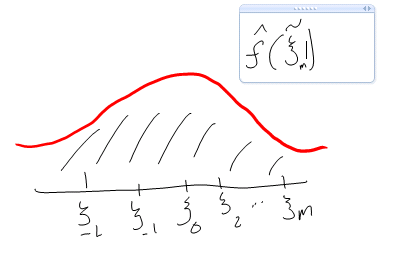
\includegraphics{10-28-2010-Reimann.png}
	\caption{Riemann Sum.}
	\label{fig:Reimann}
\end{figure}

This is the inverse Fourier Transform
$$ f(x) = \frac{1}{2 \pi} \int_{- \infty}^{\infty} \fhat(\xi) e^{i \xi x}~d\xi.$$
\subsection{Proof by example}
Suppose 
$$f(x) = \begin{cases}
1 \quad |x| \leq d\\
0 \quad |x| \geq d
\end{cases}$$
Complex Fourier Series (assume $L > d$):
$$c_m = \frac{1}{2L} \int_{-L}^L f(x) e^{-i \xi x}~dx = \frac{1}{2L} \int_{-d}^d e^{-i \xi x}~dx = \frac{2\sin(\frac{m \pi d}{L})}{m \pi / L} \frac{1}{2L}.$$
So
$$ 2L c_m = \frac{2 \sin(\xt d)}{\xt} \qquad \xt = \frac{m \pi}{L}.$$
Fourier Transform:
$$ \fhat(\xi) = \int_{-\infty}^{\infty} f(x) e^{-i \xi x}~dx = \int_{-d}^d e^{-i \xi i}~dx = \frac{2 \sin(\xi d)}{\xi}.$$
Also I claim
$$ f(x) = \frac{1}{2 \pi} \int_{-\infty}^{\infty} \frac{2 \sin(\xi d)}{\xi} e^{i \xi x}~dx.$$
The proof of this is left to the reader.
\section{Is the Fourier Transform Useful?}
Yes. The Fourier Transform can be used to solve ODEs and PDEs.
\subsection{Example 1}
Compute the Fourier Transform of
$$f(x) = H(x) e^{-ax}$$
for $a > 0$, where
$$H(x) = \begin{cases} 1 \quad x > 0 \\ \frac12 \quad x = 0 \\ 0 \quad x < 0\end{cases},$$
is Heaviside function, so 
\begin{figure}
	\centering
		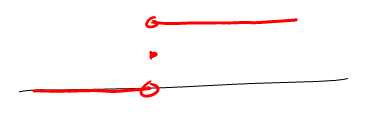
\includegraphics{10-28-2010-heaviside.png}
	\caption{The Heaviside Function.}
	\label{fig:heaviside}
\end{figure}
$$H(x)e^{-ax} = \begin{cases} e^{-ax} \quad x > 0 \\ \frac12 \quad x = 0 \\ 0 \quad x < 0 \end{cases}.$$
\begin{figure}
	\centering
		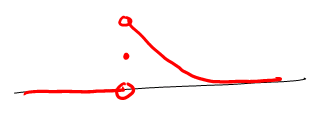
\includegraphics{10-28-2010-heavisideT.png}
	\caption{Graph of $H(x)e^{-ikx}$.}
	\label{fig:heavisideT}
\end{figure}

\begin{align*}
\mathscr \{f(x)\} &= \fhat(k) \\
&= \int_{0}^{\infty} e^{-ax} e^{-i k x} ~dx \\
&= \int_0^{\infty} e^{-(a + ik)x}~dx \\
&= \frac{e^{-(a+ik)x}}{-(a+ik)} \Big[_{x = 0}^{\infty} \\
&= \frac{1}{a + ik}.
\end{align*}
\subsection{Example 2}
Suppose $\yhat(k) = \mathscr F \{y(x) \}$, wthat can we say about $\mathscr F \{ y'(x) \}$?
$$\yhat(k) = \int_{- \infty}^{\infty} y(x) e^{-i k x}~dx$$
and
$$ \mathscr F \{y'(x)\} = \int_{-\infty}^{\infty} y'(x) e^{-i kx }~dx.$$
We integrate by parts;
\begin{align*}
y'(x) dx &= du \\
e^{-ikx} &= v \\
y(x) &= u \\
-ike^{-ikx} = dv.
\end{align*}
So
$$ \mathscr F \{y'(x)\} = y(x) e^{-ikx} \big[_{x = - \infty}^{\infty} - \int_{-\infty}^{\infty} (-ikx)e^{-ikx} y(x)~dx.$$
If $|y(x)| \to 0$ as $|x| \to \infty$ the first term vanishes.
$$\mathscr F \{ y'(x) \} = ik \int_{- \infty}^{\infty} e^{-ikx} y(x)~dx = ik \yhat(k),$$
the Fourier Transform turns differentiation into multiplication!
\subsection{Example 3}
Solve
\begin{align*}
\text{DE:}&~y'+y = H(x)e^{-2x} \qquad - \infty < x < \infty \\
\text{DC:}&~|y(x)| \to 0 \qquad \text{as } x \to \pm \infty.
\end{align*}
Solution: Fourier Transform both sides
\begin{align*}
\mathscr F \{y' + y\} &= \mathscr F  \{ H(x) e^{-2x} \}\\
\mathscr F \{y'\} + \mathscr F \{y\} &= \frac{1}{2+ik}.
\end{align*}
But
\begin{align*}
\mathscr F \{y'\} &= ik \yhat \\
\mathscr F \{y\} &= \yhat
\end{align*}
so
\begin{align*}
ik\yhat &= \frac{1}{2+ik}\\
(1+ik)\yhat &= \frac{1}{2+ik}
\end{align*}
So
$$\yhat = \frac{1}{(1 + ik)}\frac{1}{(2+ik)}$$
But
\begin{align*}
y(x) &= \mathscr F^{-1} \{\yhat(k)\} \\
&= \mathscr F^{-1} \{\frac{1}{(1+ik)}\frac{1}{(2+ik)}\}\\
&= \mathscr F^{-1} \{\frac{1}{1+ik} - \frac{1}{2+ik}\} \\
&= H(x)e^{-x} - H(x)e^{-2x}.
\end{align*}
So
$$y(x) = H(x)[e^{-x}-e^{-2x}].$$ 
\begin{figure}
	\centering
		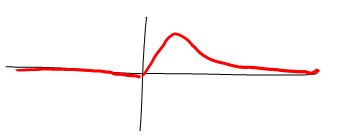
\includegraphics{10-28-2010-soln.png}
	\caption{Sketch of the solution.}
	\label{fig:soln}
\end{figure}

\section{Transform of the Delta Function}
$$\mathscr F \{\delta(x)\} = \int_{-\infty}^{\infty} \delta(x) e^{-ikx}~dx = 1.$$
\end{document}